%%%%%%%%%%%%%%%%%%%%%%%%%%%%%%%
%% Folie: DataGen            %%
%%%%%%%%%%%%%%%%%%%%%%%%%%%%%%%

\begin{frame}
    \frametitle{Data Generation}

\vspace*{1cm}
\begin{multicols}{2}
	\begin{PraesentationAufzaehlung}
	
	\item Airfoil shapes from UIUC database

    \item Reynolds number: $[0.5, 5] \cdot 10^6$ (highly turbulent)

    \item Angle of attack: $[-22.5, 22.5]$

    \item Ground truth generated with OpenFOAM \newline (pressure, x velocity, y velocity)
    
    \item Training data resolution: $3\times 128 \times 128$ \newline (Inference region $<$ full simulation domain)
    \end{PraesentationAufzaehlung}
    \vfill\columnbreak
    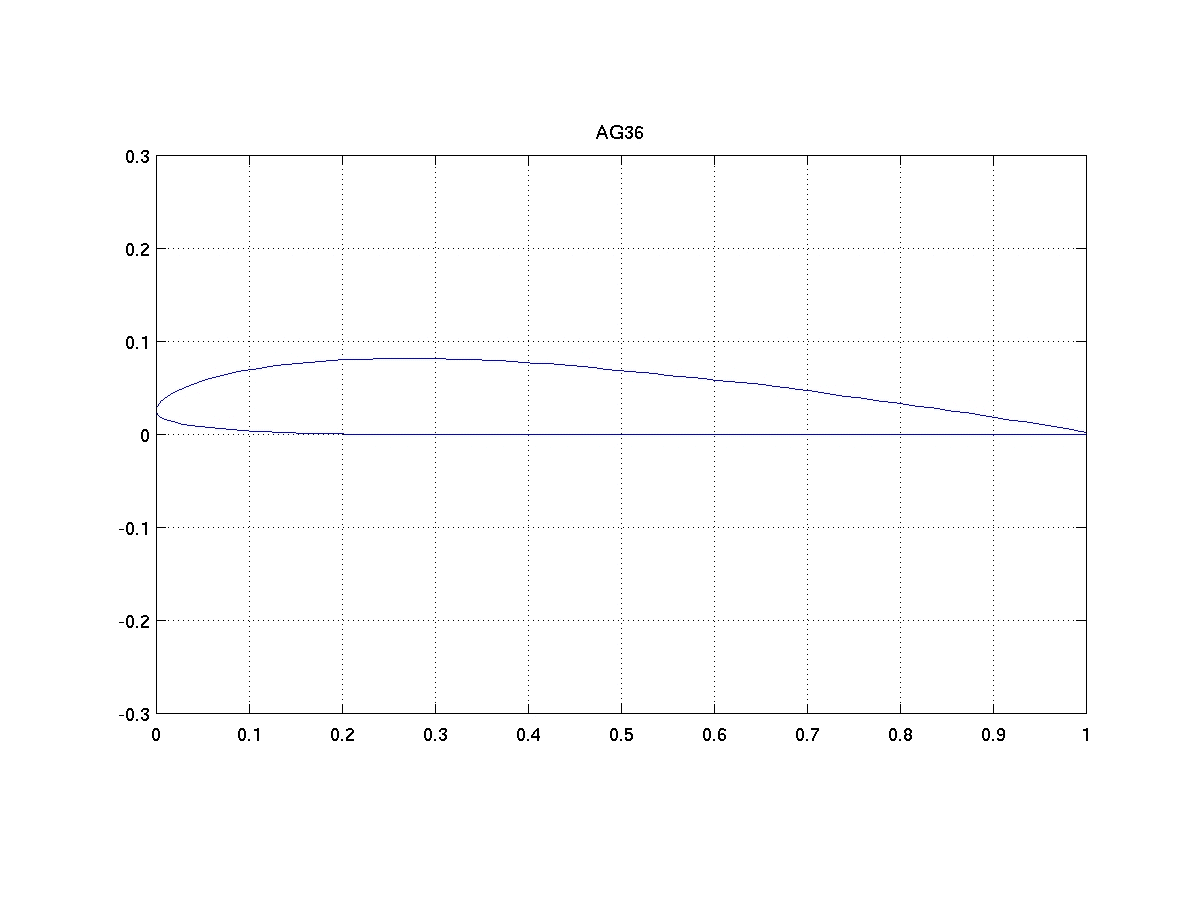
\includegraphics[width=\columnwidth, height=.6\textheight]{./Ressourcen/Praesentation/Bilder/uiuc_sample.png}
    
\end{multicols}
	\vspace*{-1.4cm}
    Taken from \url{https://m-selig.ae.illinois.edu/ads/afplots/ag35.gif}
\end{frame}
\clearpage